\documentclass[xetex,mathsans,sans,aspectratio=169]{beamer}
\usepackage{listings}
\usetheme{Boadilla}
\usecolortheme{orchid}
\usepackage{fontspec}
\setsansfont{Basis Grotesque}
\setbeamertemplate{navigation symbols}{}


\title[NuCypher KMS]{NuCypher KMS: Decentralized Key-Management System}
\author[Michael]{Michael Egorov, CTO}
\date[15 Feb 2018]{ETHDenver, 15 Feb 2018}

\begin{document}
    \begin{frame}
        \titlepage
        \begin{figure}
            \centering
            
\includegraphics[width=5cm]{pdf/nucypher_logo.pdf}
        \end{figure}
    \end{frame}

    \begin{frame}
        \frametitle{Why}
        \framesubtitle{Encrypted file sharing}
        \begin{figure}
            \centering
            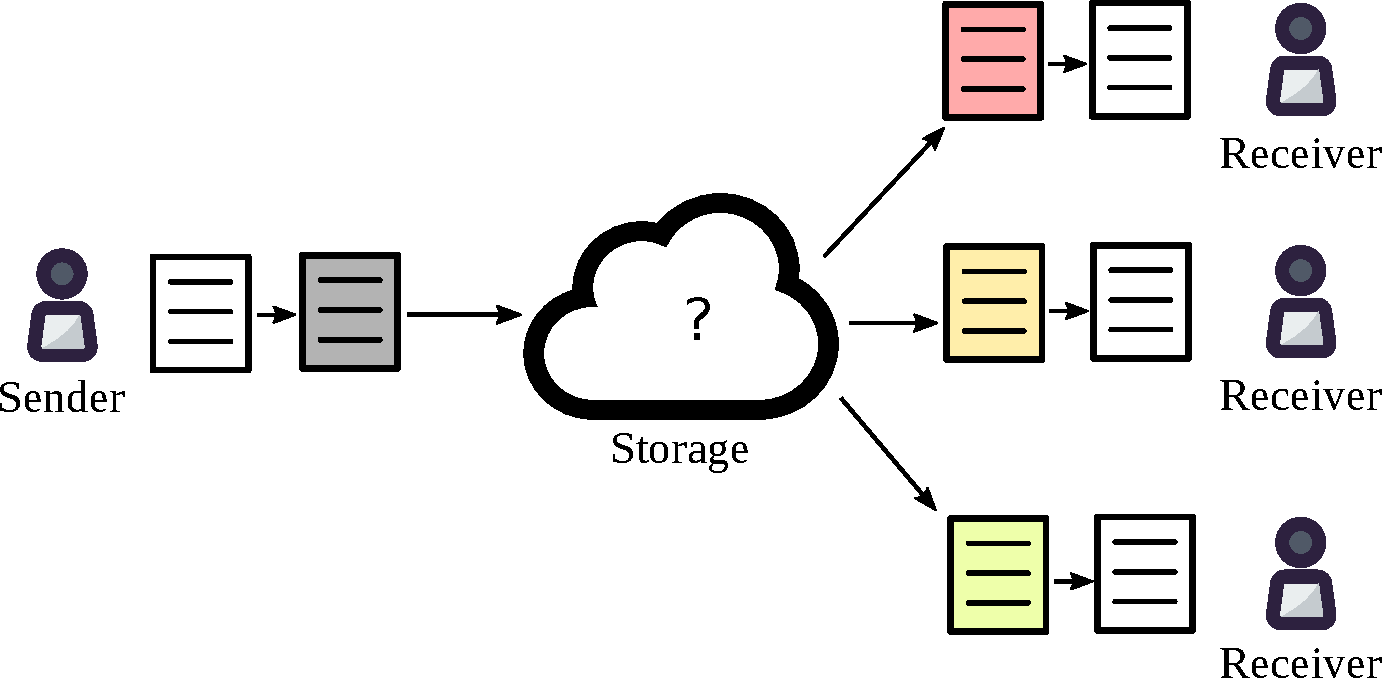
\includegraphics[height=5.5cm]{pdf/file-sharing.pdf}
        \end{figure}
    \end{frame}

    \begin{frame}
        \frametitle{Why}
        \framesubtitle{Encrypted multi-user chats}
        \begin{figure}
            \centering
            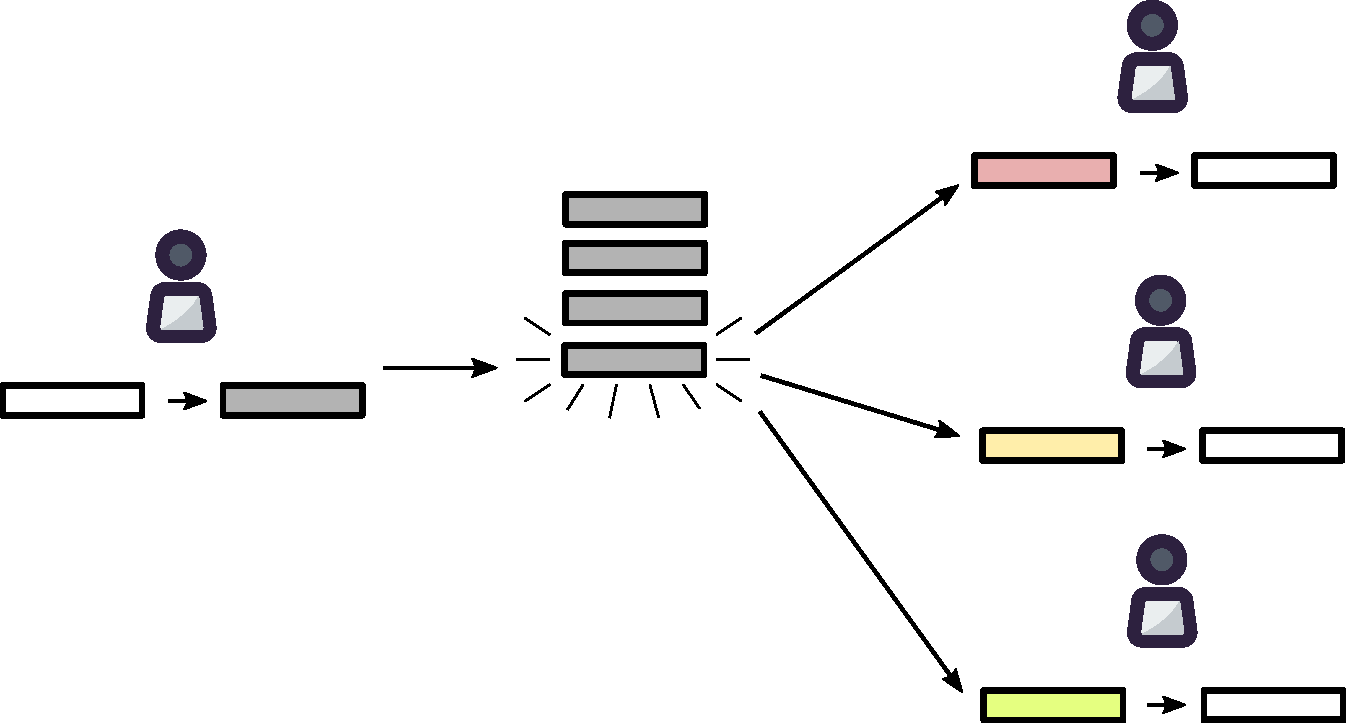
\includegraphics[height=5.5cm]{pdf/chats.pdf}
        \end{figure}
    \end{frame}

    \begin{frame}
        \frametitle{Why}
        \framesubtitle{Decentralized Netflix}
        \begin{figure}
            \centering
            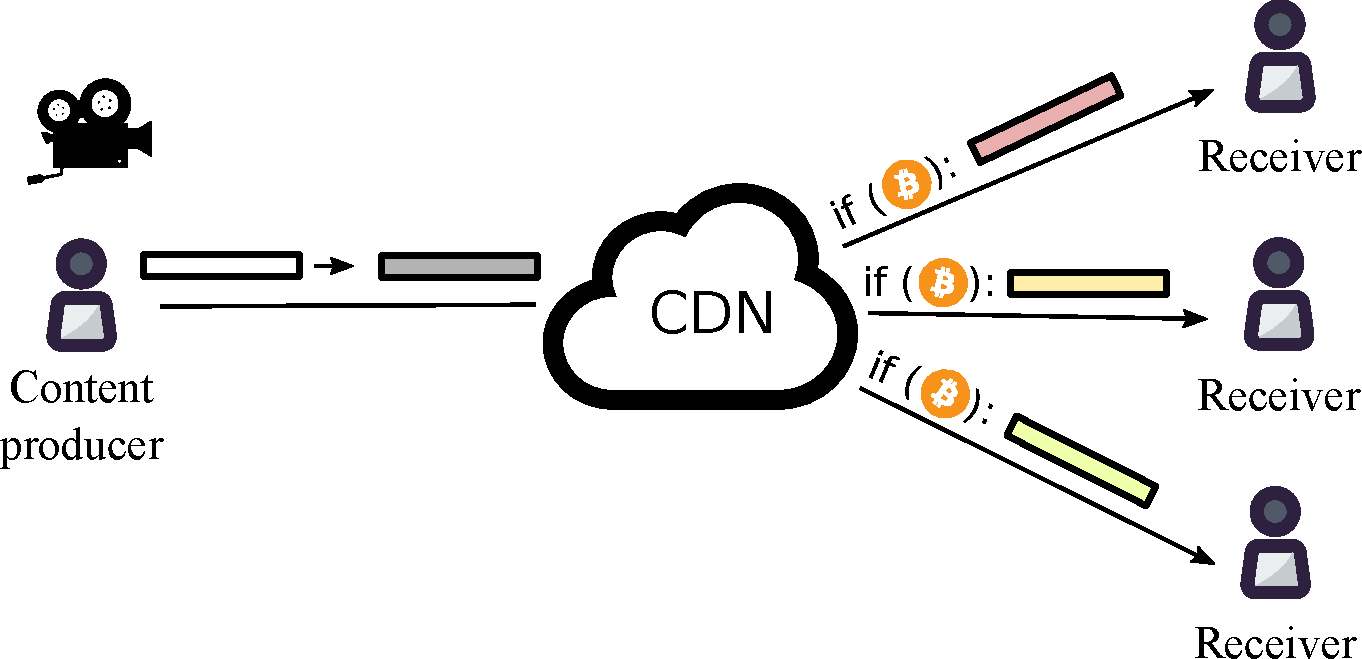
\includegraphics[height=5.5cm]{pdf/streams.pdf}
        \end{figure}
    \end{frame}

    \begin{frame}
        \frametitle{Central server + TLS}
        \framesubtitle{Data vulnerable to hackers, state actors etc}
        \begin{figure}
            \centering
            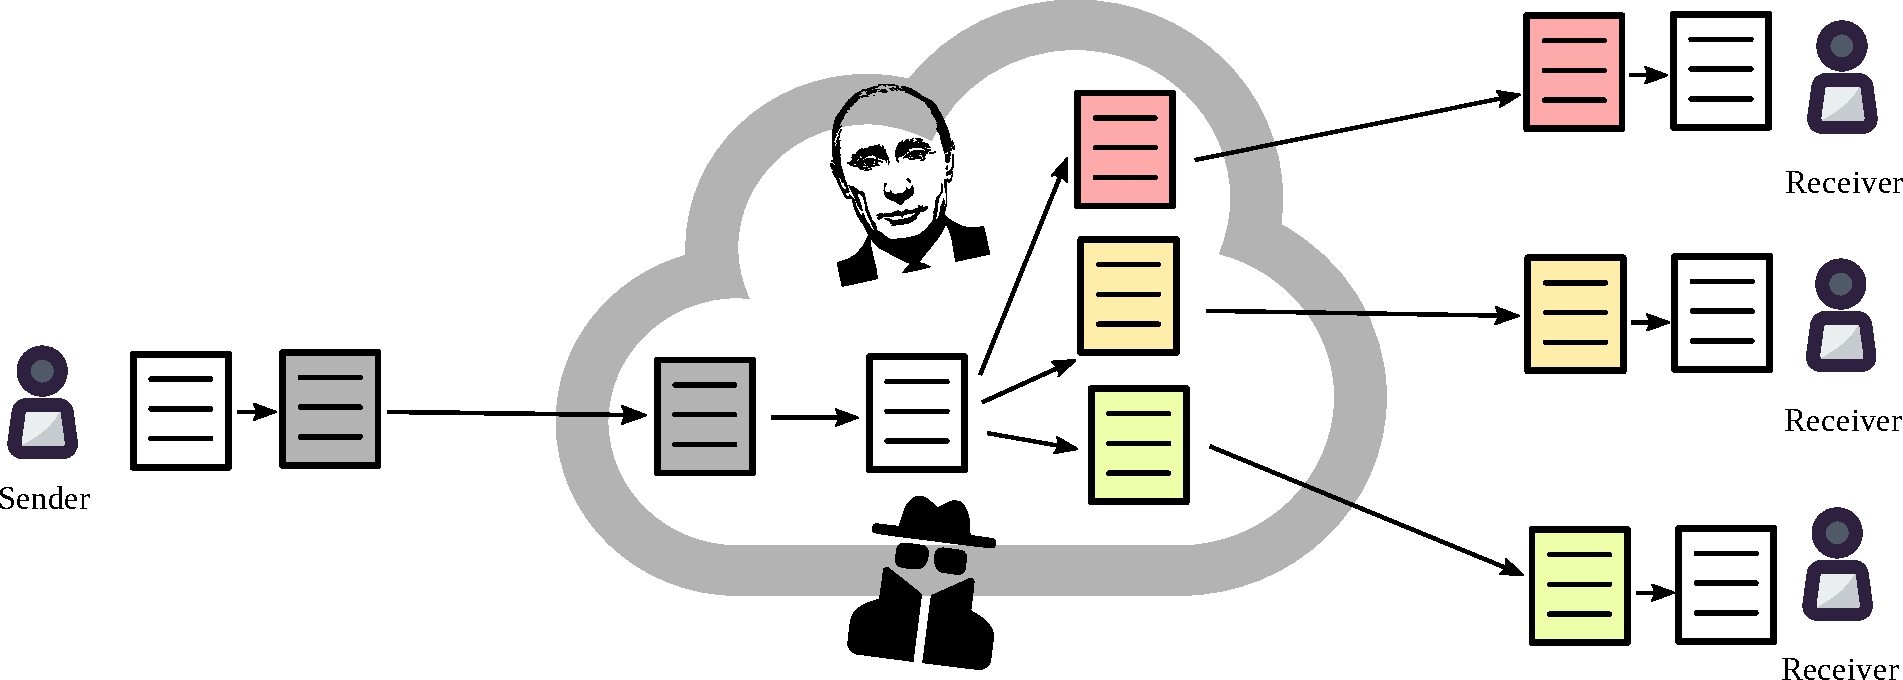
\includegraphics[width=11cm]{pdf/file-sharing-tls.pdf}
        \end{figure}
    \end{frame}

    \begin{frame}
        \frametitle{Solution}
        \framesubtitle{Proxy re-encryption + decentralization}
        \begin{figure}
            \centering
            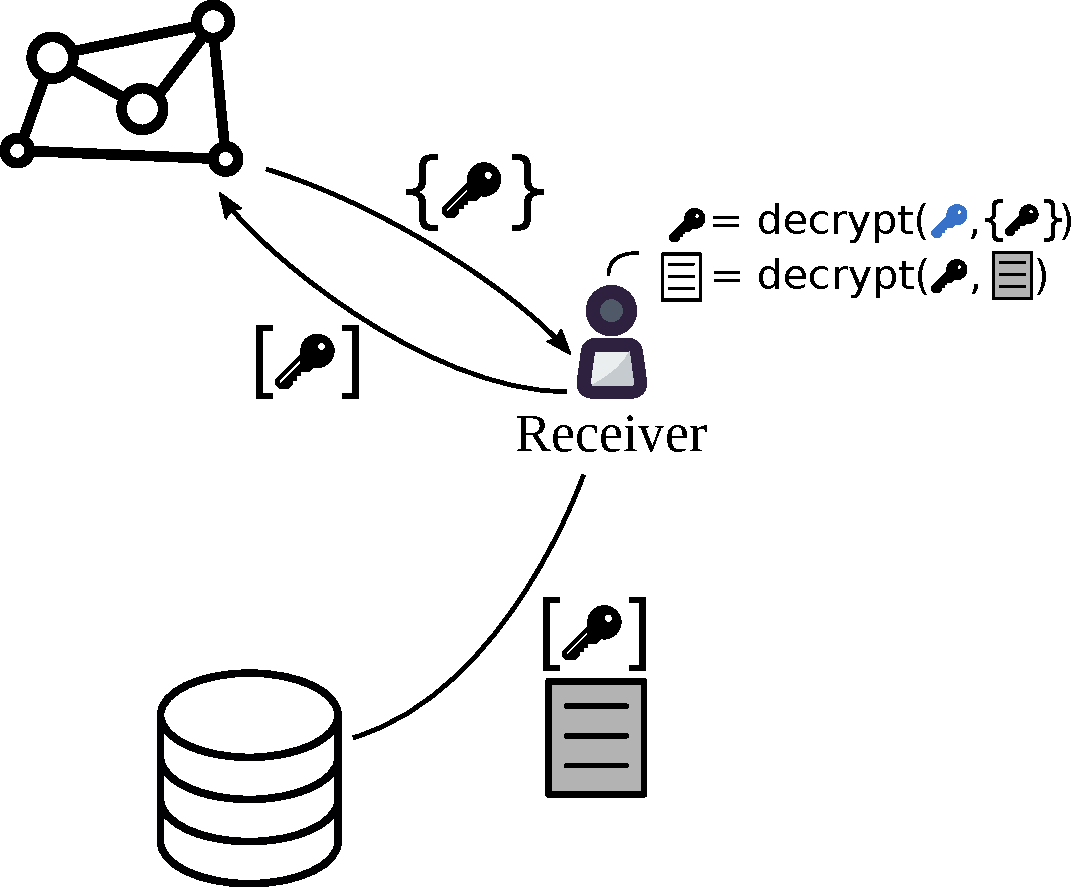
\includegraphics[height=5.5cm]{pdf/pre-kms.pdf}
        \end{figure}
    \end{frame}

    \begin{frame}
        \frametitle{What is proxy re-encryption (PRE)}
        \begin{figure}
            \centering
            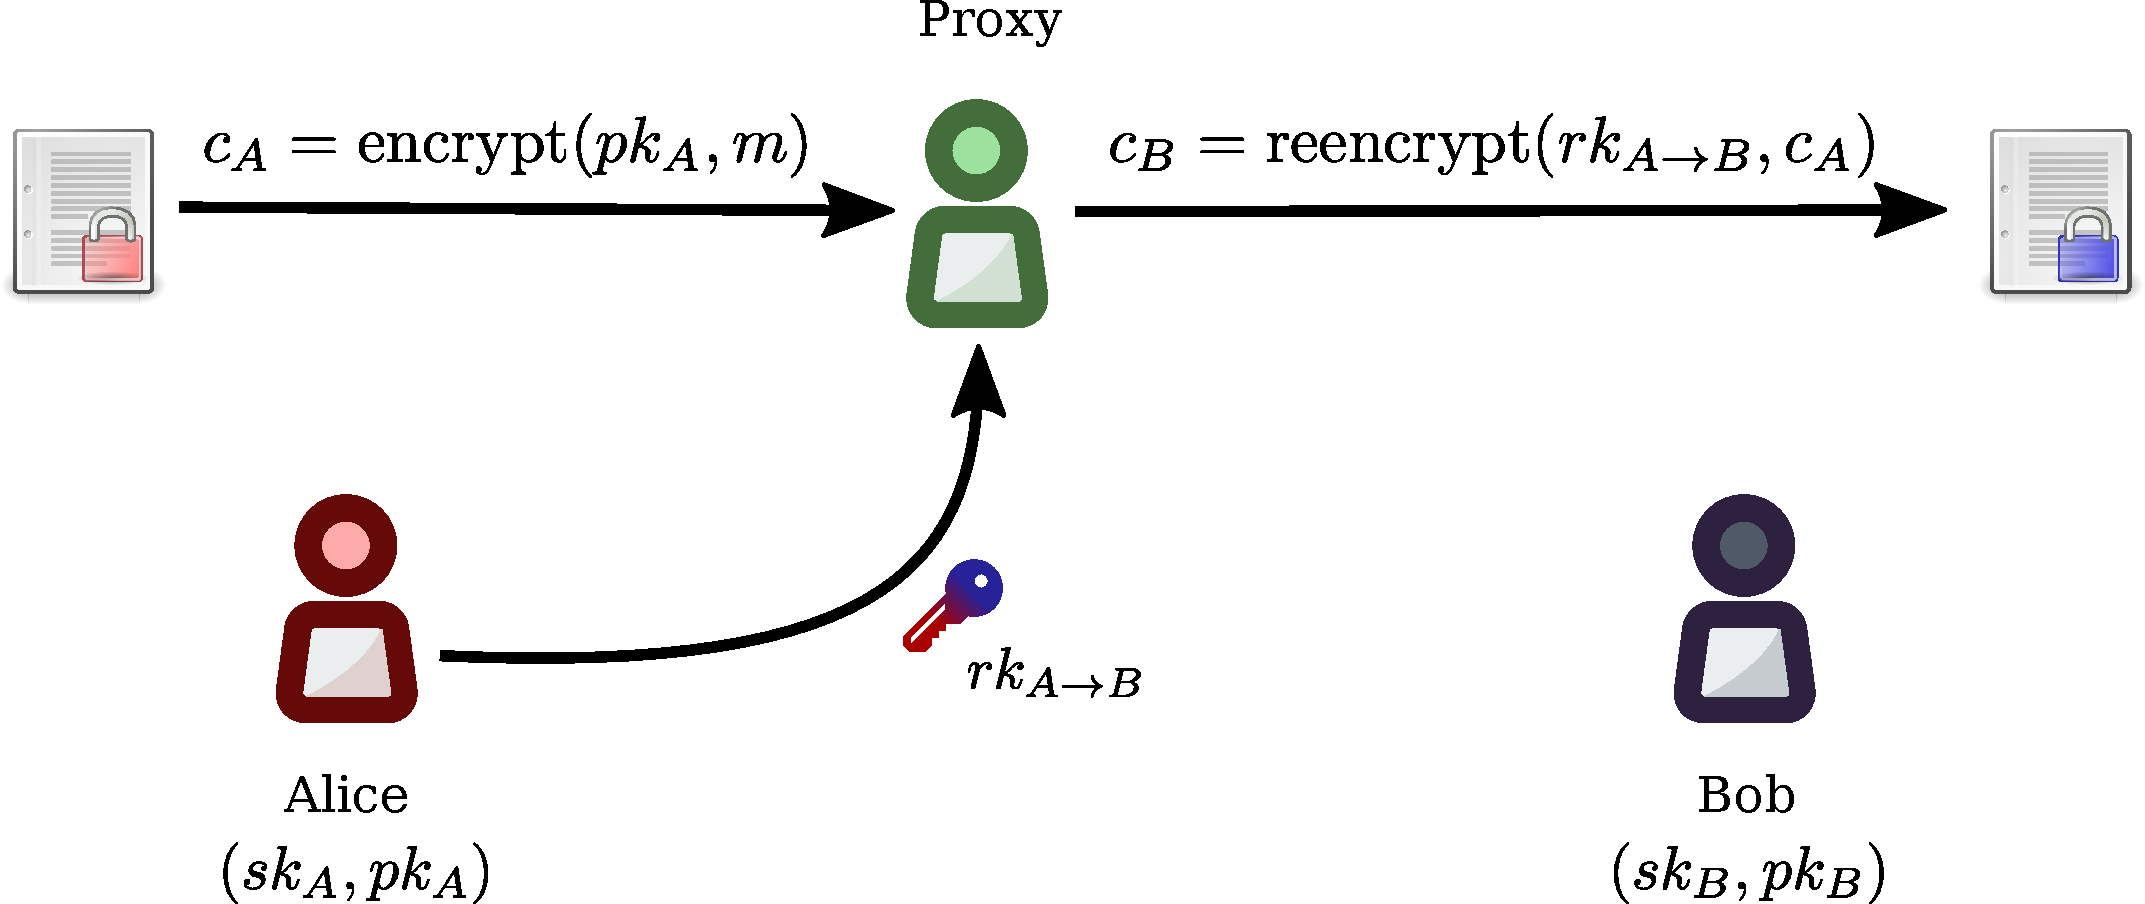
\includegraphics[width=11cm]{pdf/pre.pdf}
        \end{figure}
    \end{frame}

    \begin{frame}
        \frametitle{Centralized KMS using PRE}
        \framesubtitle{Encryption}
        \begin{figure}
            \centering
            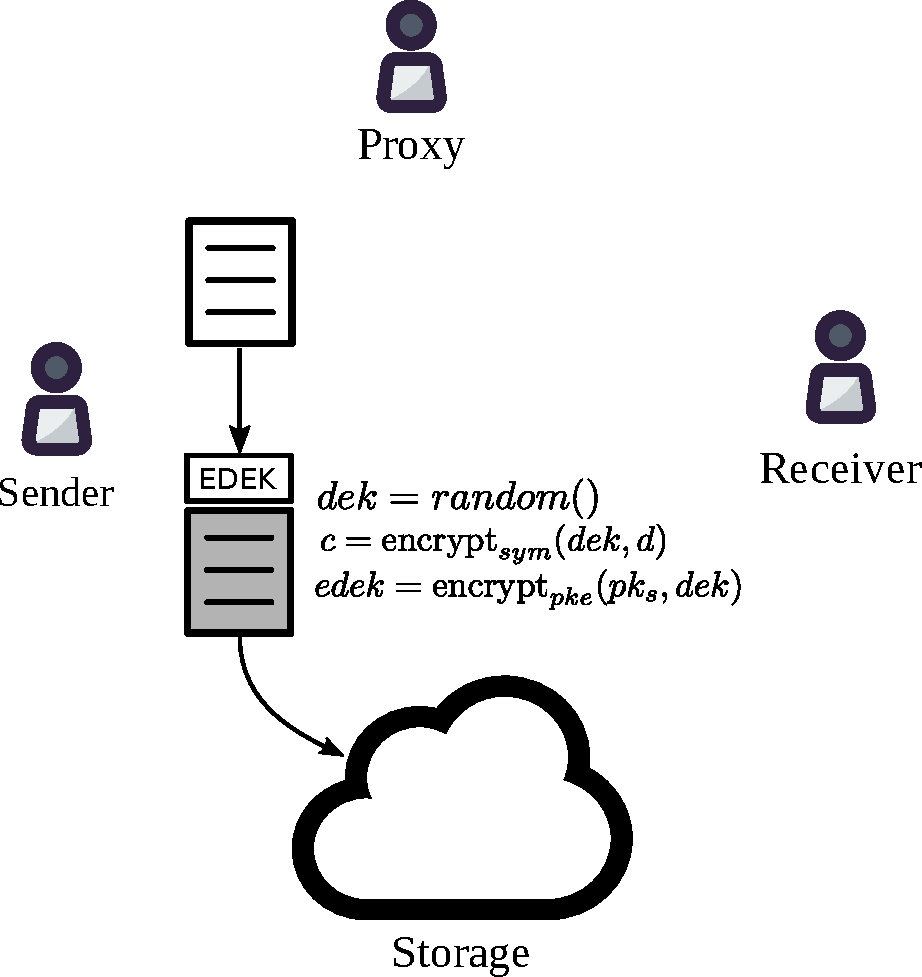
\includegraphics[height=5.5cm]{pdf/encrypt.pdf}
        \end{figure}
    \end{frame}

    \begin{frame}
        \frametitle{Centralized KMS using PRE}
        \framesubtitle{Access delegation}
        \begin{figure}
            \centering
            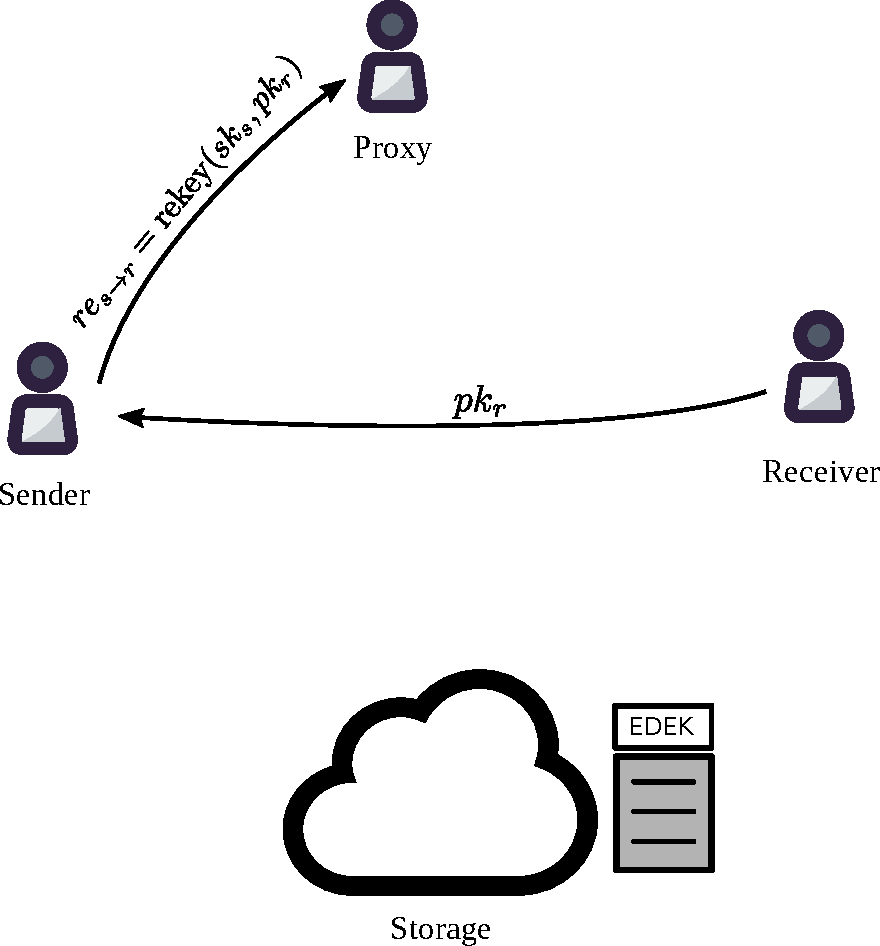
\includegraphics[height=5.5cm]{pdf/delegate.pdf}
        \end{figure}
    \end{frame}

    \begin{frame}
        \frametitle{Centralized KMS using PRE}
        \framesubtitle{Decryption}
        \begin{figure}
            \centering
            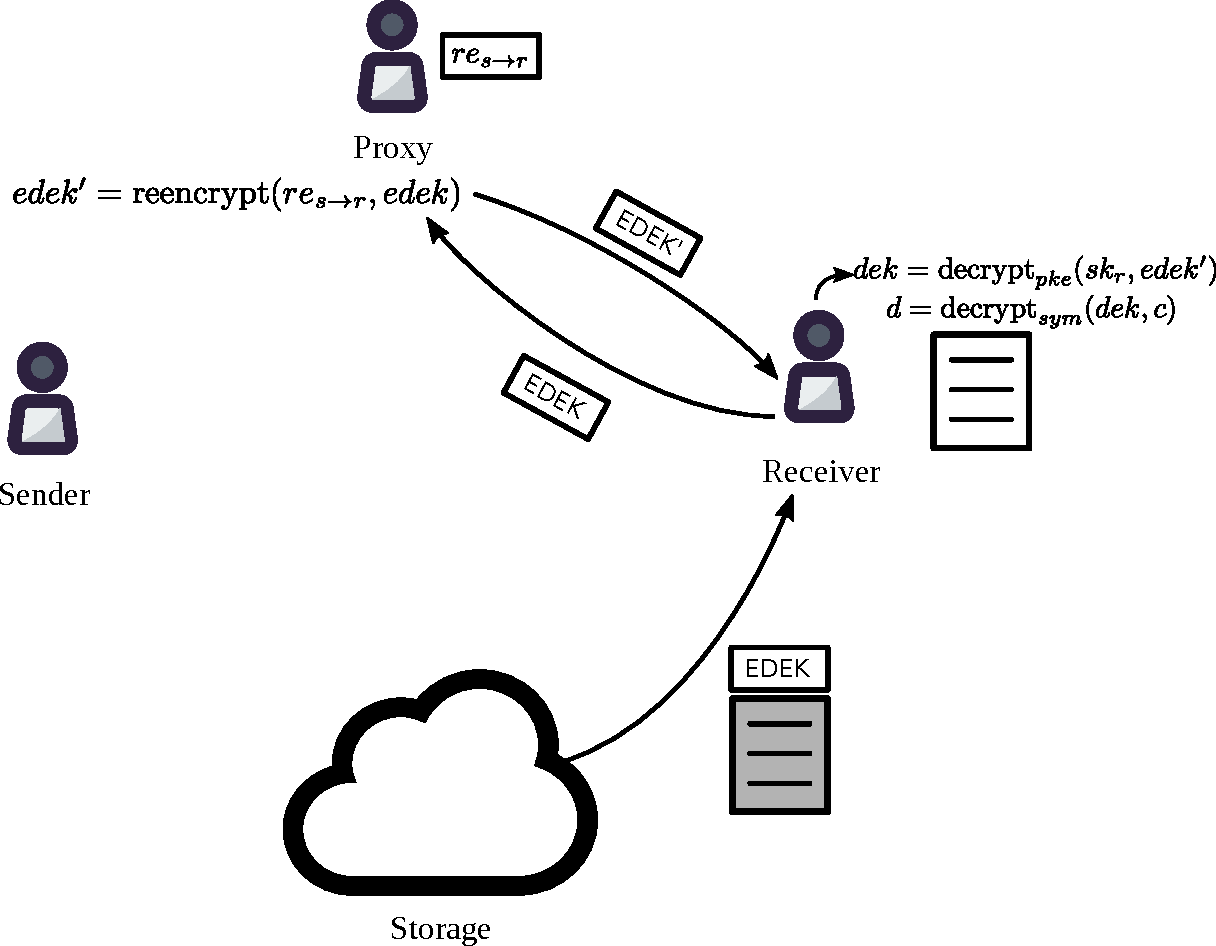
\includegraphics[height=5.5cm]{pdf/decrypt.pdf}
        \end{figure}
    \end{frame}

    \begin{frame}
        \frametitle{Decentralized key management}
        \framesubtitle{Using threshold split-key re-encryption (Umbral)}
        \begin{figure}
            \centering
            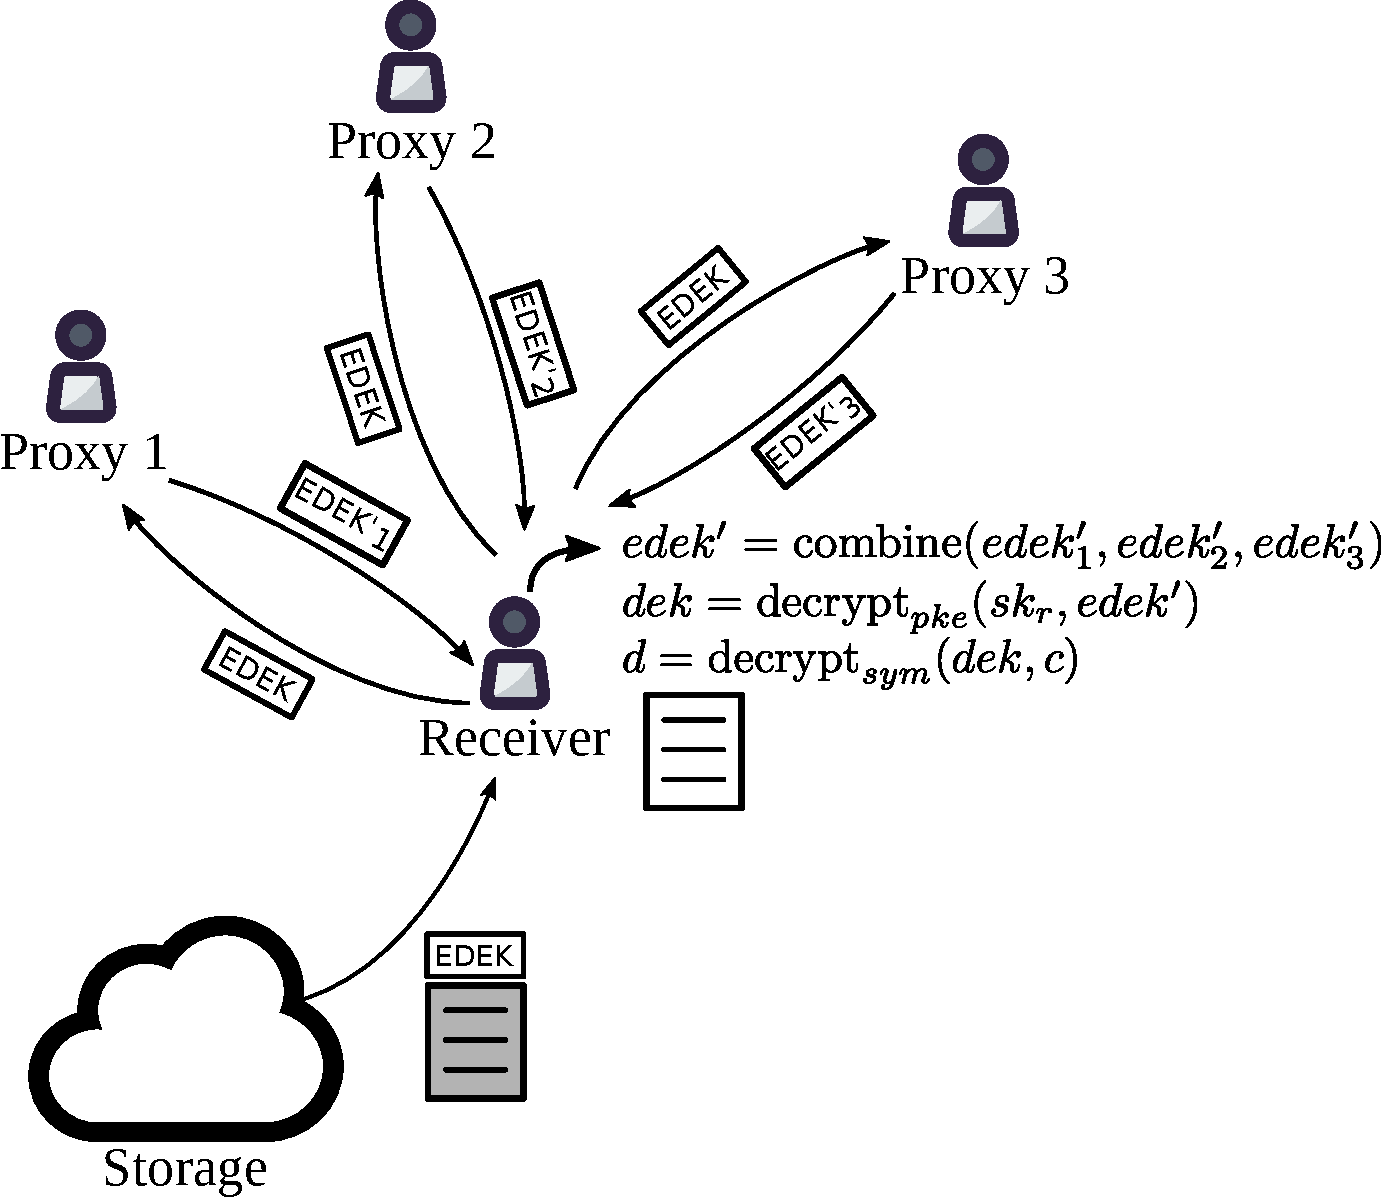
\includegraphics[height=6.5cm]{pdf/decrypt-umbral.pdf}
        \end{figure}
        \url{https://github.com/nucypher/nucypher-kms/}
        \url{https://github.com/nucypher/pyUmbral/}
    \end{frame}

    \begin{frame}
        \frametitle{Umbral: Threshold Proxy Re-Encryption}
        %\framesubtitle{Purpose}
        \begin{itemize}
        	\item \emph{``Umbral''} is Spanish for \emph{``threshold''}
            \item PRE properties: Unidirectional, single-hop, non-interactive
            \item It follows a KEM/DEM approach:
            	\begin{itemize}
					\item UmbralKEM provides the threshold re-encryption capability
            		\item The DEM can be any authenticated encryption (currently ChaCha20-Poly1305)
        		\end{itemize}
			\item IND-PRE-CCA security
			\item Verification of re-encryption correctness through Non-Interactive ZK Proofs of Knowledge
			\item Code: \url{https://github.com/nucypher/pyUmbral/}
			\item Documentation (WIP): \url{https://github.com/nucypher/umbral-doc}
        \end{itemize}
    \end{frame}

    \begin{frame}
        \frametitle{PRE demo}
        \begin{figure}
            \centering
            
\includegraphics[height=5.5cm]{pdf/terminal.pdf}
        \end{figure}
    \end{frame}

    \begin{frame}
        \frametitle{KMS token}
        \framesubtitle{Purpose}
        \begin{itemize}
            \item Splitting trust between re-encryption nodes (more tokens = more trust and more work);
            \item In-network means of payment for deploying policies;
            \item Proof of Stake for minting new coins according to the mining schedule;
            \item Security deposit to be at stake against malicious behavior of nodes
        \end{itemize}
    \end{frame}

    \begin{frame}
        \frametitle{KMS token}
        \framesubtitle{Mining}
        Mining reward:
        $$\text{reward} = \frac{\text{locked\_tokens} \times \text{reward\_rate}}{\sum_{\text{all miners}} {\text{locked\_tokens}}} + \sum_{\text{this miner}} {\text{miner\_fees}}$$
    \end{frame}

    \begin{frame}
        \frametitle{Usage examples}
        Decentralized marketplaces:
        \begin{itemize}
            \item Datum.
        \end{itemize}
        Decentralized databases:
        \begin{itemize}
            \item Bluzelle;
            \item Fluence;
            \item Wolk.
        \end{itemize}
        Medical data sharing
        \begin{itemize}
            \item Medibloc;
            \item IRYO;
            \item Medixain;
            \item Wholesome.
        \end{itemize}
        IoT
        \begin{itemize}
            \item Spherity (together with BigchainDB).
        \end{itemize}
        Cryptocurrency keys
        \begin{itemize}
            \item Coval Emblem Vault
        \end{itemize}
    \end{frame}

    \begin{frame}
        \frametitle{Useful links}
        \begin{figure}
            \centering
            
\includegraphics[width=5cm]{pdf/nucypher_logo.pdf}
        \end{figure}
        Website: \url{https://nucypher.com/blockchain.html}

        Github: \url{https://github.com/nucypher/}

        PyUmbral on Github: \url{https://github.com/nucypher/pyUmbral/}

        Slack: \url{https://nucypher-kms-slack.herokuapp.com/}

        Whitepaper: \url{https://arxiv.org/abs/1707.06140}

        E-mail: \url{michael@nucypher.com}
    \end{frame}
\end{document}

